% !TeX spellcheck = <engl>
\let\textcircled=\pgftextcircled


\chapter{Implementation}
\label{chap:implementation}

Following the prior discussion, this section seeks to address three challenges affecting affecting object detection models for AVs. This will be necessary to achieve the objectives outlined. Firstly, the necessary datasets to be used for the different evaluation tasks will be outlined . The second task will be to determine whether it is possible to detect the context of  images/point clouds from their features. Upon successful classification of images/pointclouds into their respective contexts, the performance of multimodal and LiDAR in different contexts will be assessed.  Finally, the performance of the LiDAR only model will be validated using an external dataset to determine if indeed LiDAR based object detection models are extrapolable to different datasets. 
\section{Datasets}
\subsection{Context Classification}
\begin{enumerate}
	\item \textbf{Cityscapes} - Cityscapes is a large-scale dataset used to develop pixel and instance level semantic segmentation models. It is composed of a scenes from 50 different cities captured using stereo cameras. In 5000 scenes, the images have been annotated on a pixel-level. 20000 scenes have also been coarsely annotated. In addition to this, a benchmark suite to evaluate these models is available.  
	
	\item \textbf{KITTI Object Detection}- KITTI dataset was collected with the aim of encouraging the development of computer vision and robotic algorithms for AVs.The data was captured by a car was fitted with a number of sensors including a high resolution greyscale and colour cameras, Velodyne HDL-64 LiDAR and a GPS/IMU inertial navigation system. The vehicle was driven around a city, rural areas and highways. This dataset is available as part of a benchmark suite for various AV object detection models.The dataset consists of  a total of 14,999 images and corresponding point clouds with  7,481 as labelled training files and 7,518 being unlabelled testing files. The testing set are used for evaluating results through the official test server. However, the test server is not available for general public use. 
\end{enumerate}

\subsection{LiDAR Performance Evaluation}

\begin{enumerate}
	\item \textbf{University of Bristol Smart Internet Lab(SIL)} - This dataset was captured from a  Velodyne VLP-16 LiDAR on stationary vehicle positioned at the Millennium Square in Bristol as part of the connected and autonomous vehicles project. Available as LiDAR network capture files(.pcap).
	\item \textbf{KITTI Object Detection}
\end{enumerate}

\section{Can We Automatically Detect The  Context in Driving Scenes?}

Determining the context from images and point clouds where no prior information about their location nor context  has been provided is quite difficult. This is often the case in a lab setting where the data is obtained from public database. This was indeed the case with images and point clouds from the KITTI dataset that did contain such information and since the  frames were discontinuous as they shuffled into training and testing sets, it was difficult to infer the context using the sequence of prior frames. Notably, this was also evident in the Cityscapes dataset. From this observation, it was necessary to create a context detector for images and furthermore point clouds that can be used in a lab setting. 
%. As a result there was no way to determine the context aside from visual examination of images.
%This was the intuition for creating a context detector that can be used in a lab setting by researchers looking to understand processes in  different contexts. 

% In mowhere you are able to infer from a map. However in a lab setting where you are only using image data from datasets this becomes quite difficult. This is mostly due to loss of spatio-temporal information if not prior specified or if so, done coarsely. Both VoxelNet and AVOD models were trained using the KITTI data. The frames were discontinuous and shuffled into training and testing directories. As such it was difficult to infer the context of the frames prior as no information was provided about the location they were captured and whether it was rural or urban. Notably, this was also evident in the CityScapes dataset. From this observation, it was necessary to create a context detector for images and furthermore point clouds that can be used in a lab setting. 

To begin with, I visually classified 3749 images from the KITTI dataset to be used as training and test data for the context detector. Of these 1029 were non-urban and the remaining 2720 urban. 
The context of the image scenes were determined using the following criteria defined by the UK Department for Environment, Food \& Rural Affairs \cite{2011ruralurbanclassification}
\noindent
Urban regions are characterised by:
\begin{enumerate}
	\item High density of road users often including pedestrians, cyclists and vehicles. 
	\item Presence of numerous  buildings that tend to be large and multi-story. 
	\item Presence of multiple transport facilities such as trams. 
\end{enumerate}

\noindent
Non-urban regions are characterised by: 
\begin{enumerate}
	\item Low/medium density of road users mostly vehicles.
	\item Few or no buildings, mostly isolated dwellings.
	\item Long stretches of motorways surrounded by vegetation. 
\end{enumerate}

Following this, the classified data was split on a 80:20 ratio to be used as the training and test set respectively. 

\begin{figure}[h]
	\centering
	\begin{minipage}[b]{0.4\textwidth}
		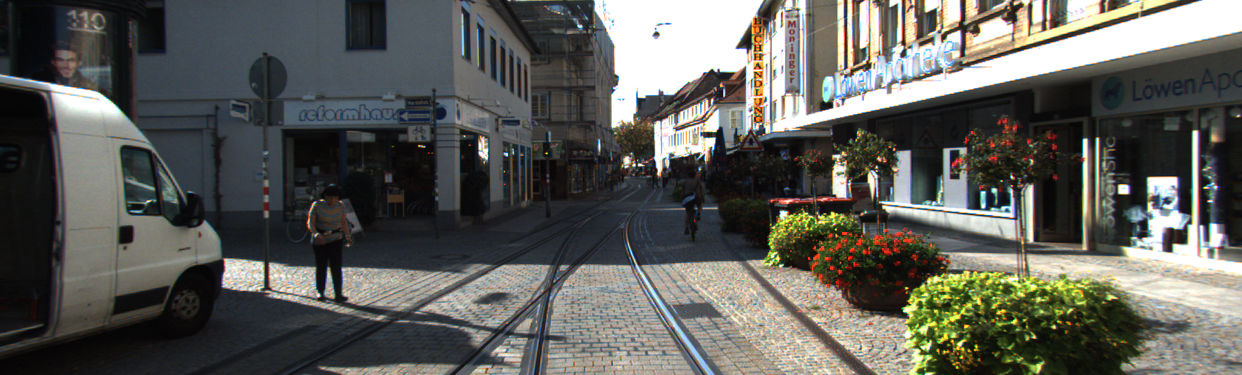
\includegraphics[width=\textwidth]{images/urban.png}
		\caption{Urban scene}
	\end{minipage}
	\hfill
	\begin{minipage}[b]{0.4\textwidth}
		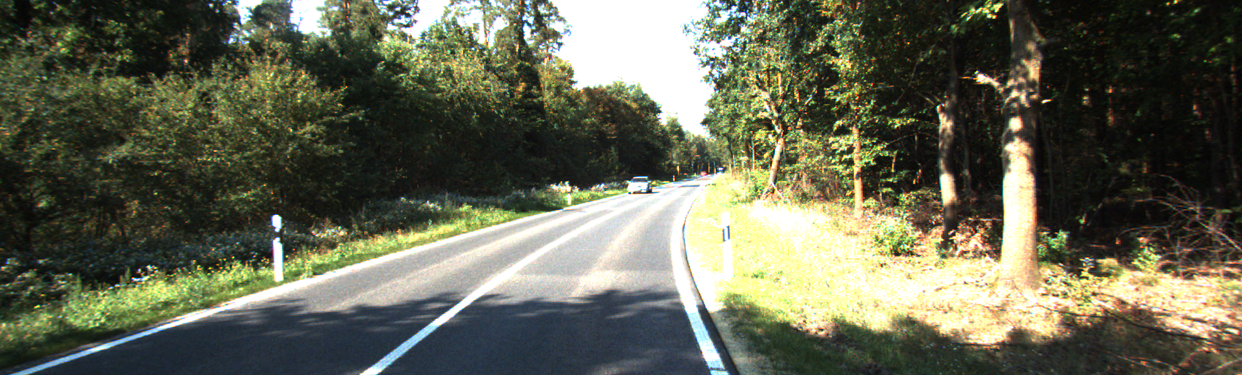
\includegraphics[width=\textwidth]{images/non_urban.png}
		\caption{Non-Urban scene}
	\end{minipage}
\end{figure}


\subsection{Image Context Detection}

Images provide a rich representation of a scene that can be exploited through image segmentation. Various image segmentation models have been developed to break down images into coherent regions.Semantic segmentation involves classifying these regions into various classes on a pixel level. 
Classic computer vision techniques for semantic segmentation utilised Texton Forests\cite{shotton2008semantic} and Random Forest classifiers \cite{shotton2011real}, however, deep learning techniques have overtaken them in terms of performance. 
Developed by Google,  Deeplab-V3 is one of the best performing open-source models on the Cityscapes semantic segmentation benchmark table. 

\subsection*{Implementation Details}


\paragraph{Extracting Semantic Histograms} Using the Deeplab-V3 network, I performed semantic segmentation on the classified images. For each image, a semantic histogram containing the number of pixels in each semantic class as seen in figure \ref{fig:sem_hist} was calculated. 


\begin{figure}[h]%
	\centering
	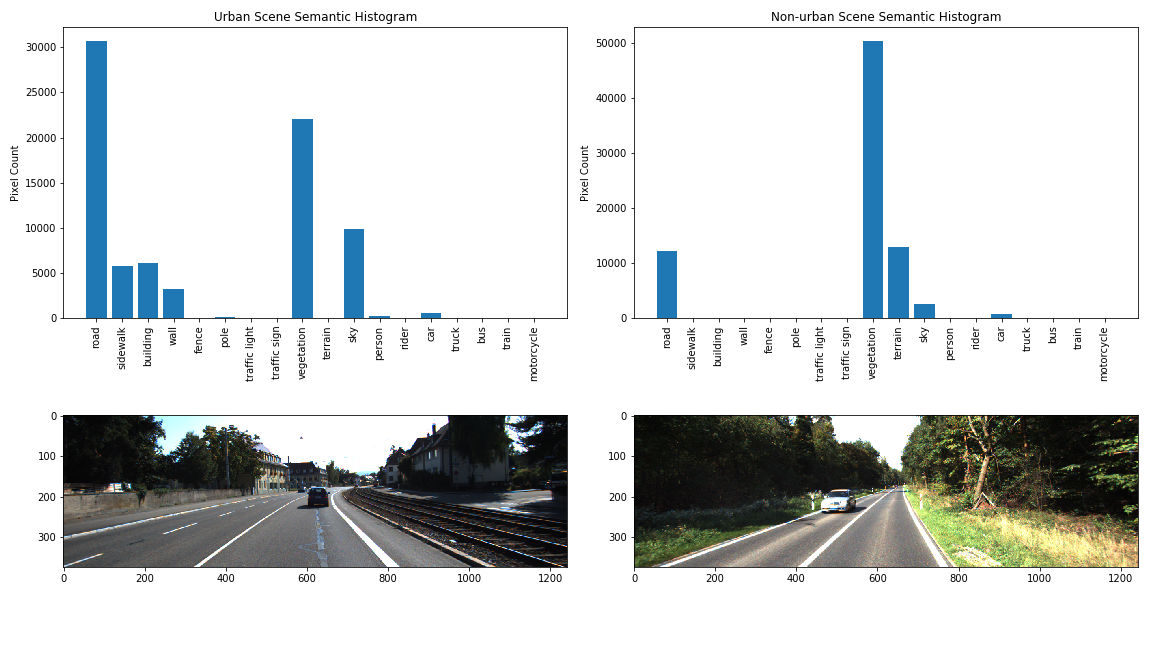
\includegraphics[width=\linewidth]{images/semantic_hist.png}%
	\caption{Semantic Histograms}%
	\label{fig:sem_hist}%
\end{figure} 

\paragraph{Training}By matching the semantic histograms with the context label of the image, I was able to train a Support Vector Machine(SVM) using the scikit-learn library to classify the image context. Linear and radial basis functions were tested on the SVM to evaluate their performance.
\paragraph{Evaluation} The trained SVM classifier was then used to classify keypoint descriptors that were extracted from the test point clouds. Given that a single point clouds can contain various features, majority voting was used to establish the dominant feature class. 

\paragraph{Penalising misclassifications} In a realistic setting, I speculated that it would be more costly to classify urban as non-urban than non-urban. This is because non-urban settings are less dynamic than urban settings. In order to extend this as part of the AV system, it was important to create a penalising factor to the classifier as defined below: 

\noindent


\begin{gather*}
	R_{urban} = \lambda _{11}P(urban |x) + \lambda _{12}P(non-urban|x)  \\ 
	R_{non_urban} = \lambda_{21}P(urban|x) + \lambda _{22}P(non-urban|x)\\ 
	Context=\left\{
		\begin{array}{@{}ll@{}}
		\text{Urban}, & \text{if}\ R_{urban} < R_{non-urban}  \\
		\text{Non-urban}, & \text{otherwise}
		\end{array}\right.
\end{gather*} 
where $\lambda $ is a 2x2 matrix with $\lambda_{11}$and $\lambda_{22}$ set to 0 and $\lambda_{12}$ set to 1.6 and $\lambda_{21}$ set to 1.





\subsection{PointCloud Context Detection}
As compared to point clouds from RGB-D or stereo cameras, point clouds from LiDAR lack rich features. This is due to the sparse nature of the point clouds and as a result, the resulting representation tends to have a large number of 'holes'. Despite the availability of point clouds segmentation models, there are no datasets with annotations of outdoor scenes such as Cityscapes. As such using semantic histograms to characterise scene contexts in this case would not be suitable.
A different approach was therefore used by first detecting the key points in the cloud, extracting and classifying features from them and later on matching these features in other point clouds.  

\begin{enumerate}
	\item \textbf{Keypoint extraction} \\ 
	Similar to classic image processing, key points are salient points that are not affected by any form of transformation or distortion. As such, they are distinctive and repeatable in different points-of-view.  They can either be global or local on a given surface with the former being preferred to extract 3D shape information and the latter for 3D object detection. 
	Currently, only a few 3D keypoint detectors have been proposed. That is Intrinsic Shape Signatures(ISS)\cite{zhong2009intrinsic}, NARF\cite{steder2010narf} and Uniform Sampling of point clouds in voxels.
	\item \textbf{Feature description} \\ 
	Keypoints extracted act as features that offer a robust representation of a local or global surface. In order to provide a description of features, a descriptor is used to encode the relevant surrounding of the keypoints. These include include Fast Point Feature Histograms(PFH)\cite{rusu2009fast}, Signatures of Histograms of Orientations(SHOT)\cite{salti2014shot}. 
	
	\item \textbf{Feature Matching} \\
	Once different feature descriptors have been obtained. They can used for object detection and segmentation using nearest-neighbour functions. For high dimension data as in the case of point-clouds, randomised kd-trees and FLANN are usually used to achieve decent performance. 
		
\end{enumerate}

\subsubsection{Implementation Details}
The above methods were implemented in Python using PyDriver\cite{thesisSTUDIENARBEITPlotkin} framework and Point Cloud Library. 
Point Cloud Library is an open-source project for 2D/3D image and point cloud processing. The library contains various software implementations of keypoint extractors, descriptors and feature matching functions. However, the implementations are written in C++ and the available Python wrappers are only for Python 2.7. 
PyDriver is a framework contains a suite of object detection, classification and tracking functions. In addition, it contains Cythonized wrappers to the Point Cloud Library functions necessary for keypoint detection, extraction and feature matching and can run on Python 3.x. Code is available at \url{https://github.com/lpltk/pydriver}


2000 images from the classified context database were used as training samples, and the remaining 1749 as test samples.
\paragraph{Training} Keypoints within the ground truth bounding boxes were extracted using  ISS with a salient and NonMaxSuppression(NMS) radius of 0.25. SHOT feature descriptor with a radius of 2 was applied on the keypoints to create feature descriptors. Each feature was assigned with the context class of the point cloud. An AdaBoost classifier was then trained on the feature types. 
\subsection{Implementation Issues} 

Despite being able to visually classify a large number of images, some images were difficult to classify as they exhibited characteristics from both contexts. Furthermore, due to the fact that the images was not contiguous , I was unable to infer their context by examining preceding image frames. As such, this affected the performance of both classifiers. 
\begin{figure}[H]%
	\centering
	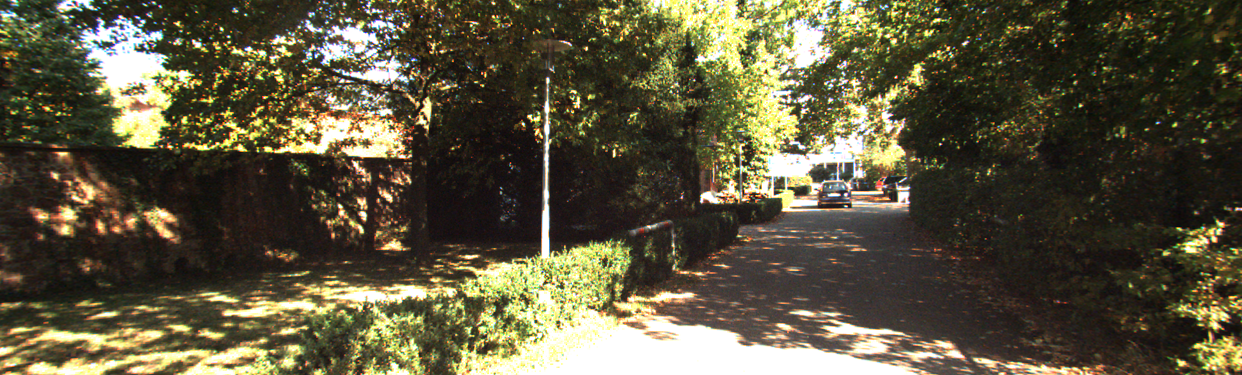
\includegraphics[width=10cm]{images/ambiguous.png}%
	\caption{Ambiguous scene}%
	\label{fig:ambiguous}%
\end{figure}

\section{ Do Some Object Detection Methods work better in Different Contexts?}

Having been able to successfully classify and create a dataset of urban and non-urban images and corresponding point clouds, the next step was evaluating how a LiDAR based and image+LiDAR based object detection model would perform in different contexts. Multimodal methods have been argued to perform better in 3D object detection tasks whereby objects are partially occluded or relatively small. Such characteristics are common in urban areas as compared to non-urban areas which have fewer and more distinct objects. In light of this argument, is it possible that LiDAR-only models can perform better or at par with multimodal methods in urban areas?

For this task,the state-of-the-art VoxelNet(LiDAR only) and AVOD(LiDAR+image) proved to be the most suitable candidates. This was influenced by the fact that they both have similar inference times, and both were open-source with the only exception being that the VoxelNet implementation was unofficial\footnote{Had similar evaluation results as the unreleased original on KITTI benchmark.}. Both of these models were written in Python and run on TensorFlow Deep Learning Framework.

\subsection{VoxelNet}
VoxelNet is an end to end point cloud based 3D object detection network that was recently published by leading researchers at Apple Inc. This network is one of the top performing LiDAR only models on the KITTI benchmark. However, the code was never released and only unofficial implementations are currently available online.
Code is available at \url{https://github.com/qianguih/voxelnet}
\subsubsection{Architecture Overview}
VoxelNet is composed of three fundamental blocks. 
\begin{enumerate}
	\item \textbf{Feature Learning Layer} \\ 
	In this layer, the point clouds are divided into equal 3D voxels. Points within these voxels are then grouped. For the car detection, 35 points are sampled and for pedestrian and cyclist detections, 35 points are sampled from within the voxels. These sampled points are then fed through multiple FCNs that learn and aggregate features from the points. The result is a 4D tensor that represents these features per voxel.
	
	\item \textbf{Convolutional Middle Layers} \\ 
	The 4D tensor containing these features is then passed through multiple convolutional middle layers. In doing so the different layers learn different features in an expanding receptive fields. This is allows the network to learn complex shape information at different scales. 
	\item \textbf{Region Proposal Network} \\ 
	Finally, the feature maps from the convolutional middle layers are fed through a RPN to classify and generate  oriented 3D bounding boxes for the objects. 
	
\end{enumerate}
\noindent
\textbf{Loss Function} 

\begin{eqnarray}
	 L & = & \alpha\frac{1}{N_{\text{\scriptsize pos}}} \sum\limits_{i} L_{\text{\scriptsize cls}}(p^{\text{\scriptsize pos}}_i, 1) + 
	\beta\frac{1}{N_{\text{\scriptsize neg}}} \sum\limits_{j} L_{\text{\scriptsize cls}}(p^{\text{\scriptsize neg}}_j, 0) \nonumber  + \frac{1}{N_{\text{\scriptsize pos}}} \sum\limits_{i} L_{\text{\scriptsize reg}}(\mathbf{u}_i, \mathbf{u}_i^*)	
	\label{eqn}
\end{eqnarray}
where:
\begin{itemize}[noitemsep]
	\item $L_{\text{\scriptsize cls}}$ is the binary cross entropy loss that is calculated for bot positive and negative classes. 
	\item $\alpha$ is a weighting parameter for the positive anchors normalised binary cross entropy loss. 
	\item $\beta$ is a weighting parameter for the negative anchors normalised binary cross entropy loss.
	\item $L_{reg}$ is the SmoothL1 regression loss.
\end{itemize}

\subsubsection{Implementation Details}
\paragraph{Training} 
To encourage generality, the model was trained on 3732 point clouds from the original KITTI training set.
VoxelNet was trained both car and pedestrian classes on two NVIDIA P100 GPUs with a batch size of 4 for 160 epochs  with $\alpha$ = 1 and  $\beta$= 10. Adam optimizer was used with an initial learning rate of 0.01 for the epochs$\le$80, 0.001 for 80$\le$epoch$\le$120 and 0.0001 for epochs$\ge$ 120. 


\paragraph{Changes to Loss Function }
In an effort to improve performance of pedestrian and cyclist detection, I implemented the focal loss function as defined in \cite{lin2018focal}. This stemmed from the fact that there were few frames with pedestrians as compared to the car class and as a result the class imbalance was high in that negative anchors $\gg$ positive anchors. 


\subsection{AVOD}
AVOD is a state of the art multimodal network that offers improved performance for small object classification by fusing LiDAR point clouds and images to perform detection. 
Code is available at \url{https://github.com/kujason/avod}
\subsubsection{Architecture Overview}
AVOD consists of three distinct stages: 
\begin{enumerate}
	
	\item \textbf{Feature Extractors } 
	
	To create a BEV map, LiDAR point clouds are projected into the XY plane and discretised to create BEV 2D grid. In each cell a height feature is defined by the maximum height of the points in the cell and it's reflectance defines the intensity feature in five slices between [0,2.5] of the Z axis. For each cell, the normalised point cloud density is calculated using $min(1.0, \frac{log(N +1)}{log 16} )$ where N is the number of points. 
	
	For the image and BEV map similat feature extractors consists of an encoder and decoder are applied. The encoder is a CNN that creates a downsampled feature map resulting in higher representation. The decoder is a Frustum Point Net that upsamples the  feature map to original size resulting in higher resolution. The output from the image and point cloud feature is fused by passing it through a 3x3 convolution layer. 
	\item \textbf{Multimodal Fusion Region Proposal Network} \\ 
	Feature maps from the point cloud and image feature extractors are fused in a RPN to generate proposals. The top proposals are then passed through a second RPN that performs object classification and bounding box regression to generate  oriented 3D bounding boxes for the objects.
\end{enumerate}

\subsubsection*{Implementation Details}

\paragraph{Training} 
Similar to VoxelNet's training method, the model was trained on 3732 point clouds  and images from the original KITTI training set. The AVOD-FPN model was trained for both car and pedestrian classes for 120000 steps on two NVIDIA P100 GPUs. The adam optimiser with an exponential decay learning rate was chosen with an initial learning rate of 0.0001 and a decay rate of 0.8 each 30000 steps. 

\begin{figure}[H]
	\centering
	\begin{minipage}[b]{0.45\textwidth}
		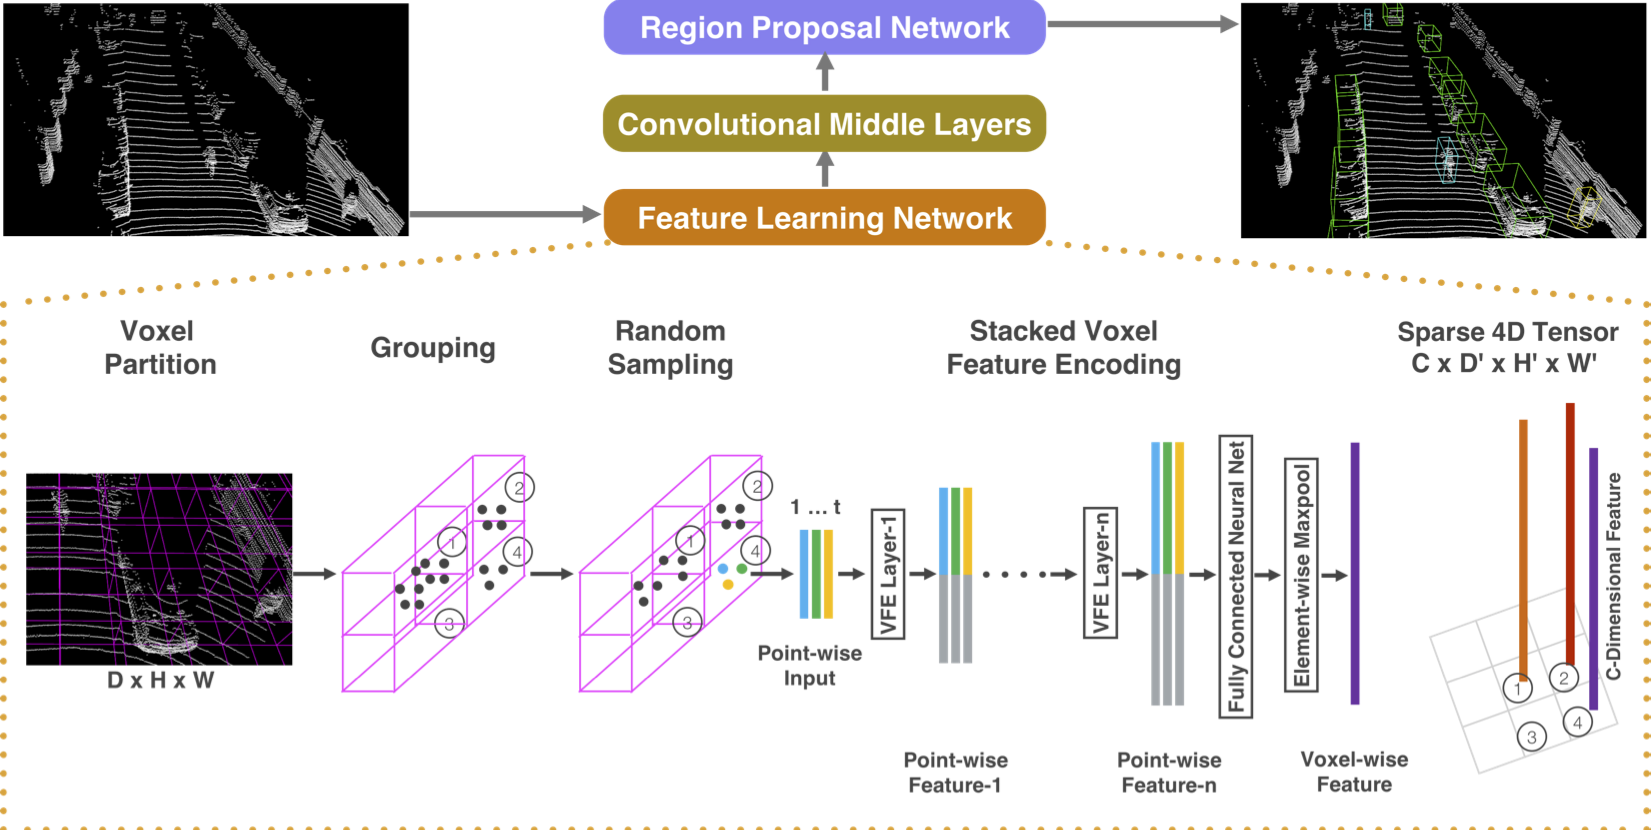
\includegraphics[width=\textwidth]{images/vox_arch.png}
		\caption{VoxelNet Architecture}
		\label{fig:voxarch}
	\end{minipage}
	\hfill
	\begin{minipage}[b]{0.45\textwidth}
		\includegraphics[width=\textwidth,height=4cm]{images/avodarch.png}
		\caption{AVOD Architecture}
		\label{fig:avodarch}
	\end{minipage}
\end{figure}


\subsection{Evaluation}

Once both models were trained, they were evaluated on 2058 images/point clouds from the context dataset with equal number of class samples. This was necessary to avoid bias as the urban samples were significantly more than the non-urban samples. For each context, each model was run on a single NVIDIA P100 GPU and the results of 3 runs  averaged. 

\subsection{Is VoxelNet Performance Valid for Different Datasets?}
As compared to image object detection methods that are can perform well regardless of  the input image resolution, LiDAR point clouds can vary in different scenes. This can depend on various factors but is largely determined by the LiDAR sensor and it's frequency in terms of points per second. Coupled with the sparse nature of point clouds, this implies that LiDAR only models may not be able to generalise to input from different LiDAR sensors with different frequencies. I  therefore set out to understand how LiDAR sensors with different frequencies affect the performance of VoxelNet
In this section I aim to validate the VoxelNet model using the SIL dataset that was obtained from a Velodyne VLP-16 sensor with a lower frequency of points than that of KITTIs Velodyne HDL-64E\footnote{See table \ref{vlp-hdl}}.
\subsubsection*{Preprocessing}
Prior to using the SIL data, I had to preprocess it to the necessary input format. 
VoxelNet only required four input fields, \textbf{XYZ values} and \textbf{reflectance} of the points, whereas the dataset was in the form of network capture files(.pcap ). To convert them into this format, I exported the capture filed into CSV format for each of the frames. This was done  in VeloView using the CSV export function. The result was a CSV file with 13 fields as seen in figure \ref{fig:sildata}

\begin{figure}[h]
	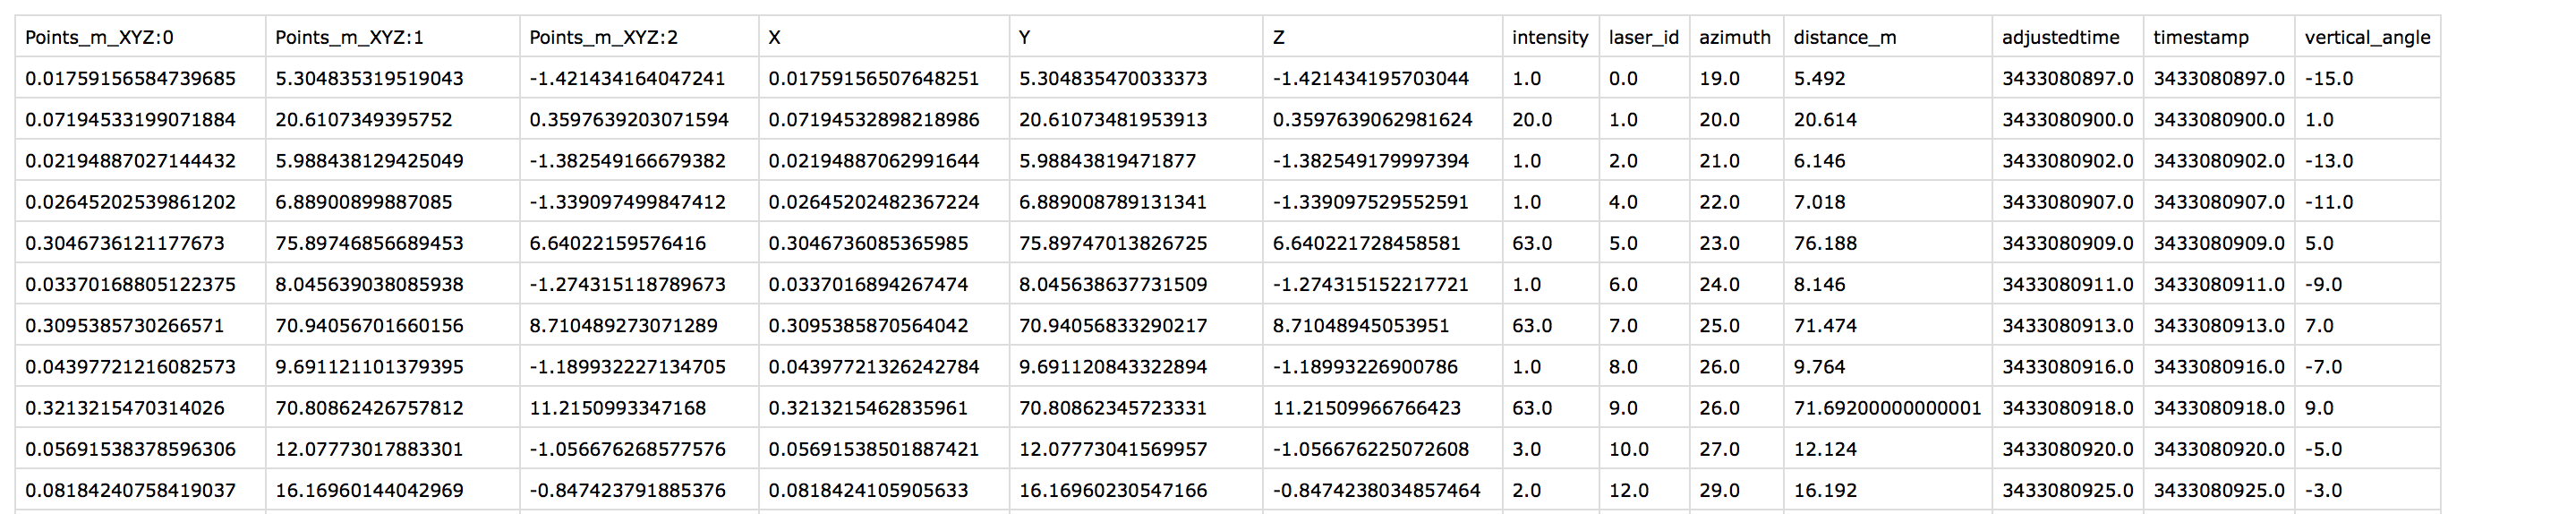
\includegraphics[width=\linewidth]{images/sildata.png}
	\caption{SIL Data Frame CSV}
	\label{fig:sildata}
\end{figure}

Out of the 13 fields, I extracted the XYZ values and intensity(reflectance) of the points and saved them as Numpy binary files. This resulted in a smaller file sizes(from around 4MB to 70KB) that are also quicker to read than normal CSV files.

\begin{figure}[h]
	\centering
	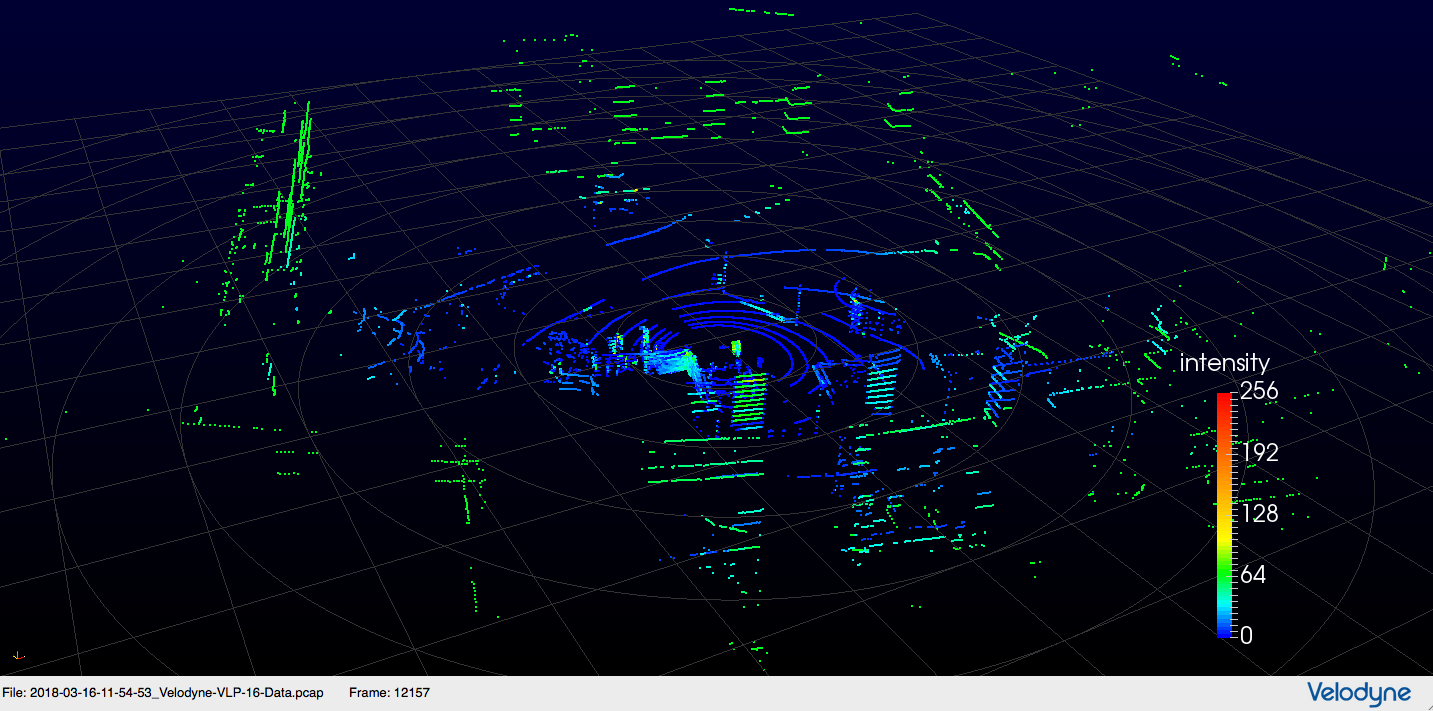
\includegraphics[width=\linewidth]{images/sil.png}
	\caption{Veloview Frame of SIL data}
	\label{fig:sil}
\end{figure}


Finally, I modified VoxelNet's configuration file to include the specifications for the VLP-16 LiDAR sensor. This was essential as the network was initially trained on KITTI point clouds that were obtained from a Velodyne HDL-64E with different specifications as seen in table \ref{vlp-hdl}. These specifications are necessary for manipulating the point clouds and therefore directly affect the performance of the network. The modified entries were the angular and vertical resolution, maximum and minimum XYZ values and the height of the VLP-16 LiDAR sensor on the vehicle. Given that there was no image data for visualisation, the image size in the configuration file was set to 0 to prevent unnecessary tensor memory allocation for images that are used for visualisation. 

\begin{table}[H]
	\centering
	\resizebox{\textwidth}{!}{%
		\begin{tabular}{|l|l|l|l|l|l|l|}
			\hline
			\textbf{LiDAR}       & \textbf{Hor FOV} & \textbf{Ver FOV} & \textbf{Range} & \textbf{Angular Resolution} & \textbf{Points/second}          & \textbf{Channels} \\ \hline
			\textit{\textbf{HDL-64E}} & 360\degree                    & 26.9\degree                 & 120m           & $\sim$0.4\degree                          & $\sim$2.2 Million                   & 64                \\ \hline
			\textit{\textbf{VLP-16}}  & 360\degree                    & $\pm$ 15\degree                 & 100m           & 0.1\degree                                & 600,000                             & 16                \\ \hline
		\end{tabular}
	}
	
	\caption{Velodyne HDL-64E and VLP-16 Specifications.}
	\label{vlp-hdl}
\end{table}



\subsubsection*{Annotating Ground Truth Labels}
The SIL dataset did not contain any ground truth labels for the point clouds as compared to the KITTI dataset. As a result, there was no metric to assess the performance of the network. To solve this, objects from the dataset needed to be annotated to obtain some ground truth bounding boxes. 

\noindent
\textbf{L-CAS Annotation Tool} \\ 
Developed by the Lincoln Centre for Autonomous Systems Research, this tool provides a semi-automatic labelling function that clusters and highlight regions of interest that may contain objects. The user can then label them depending on the object class such as car, cyclist, pedestrian. The result is then stored in a file containing the objects and their positions in the point cloud. 
To use this tool, the .pcap capture files were converted into .pcd format using the 
ROS Velodyne point cloud package\footnote{See listing \ref{lst:ros}}. 

\begin{figure}[h]
	
	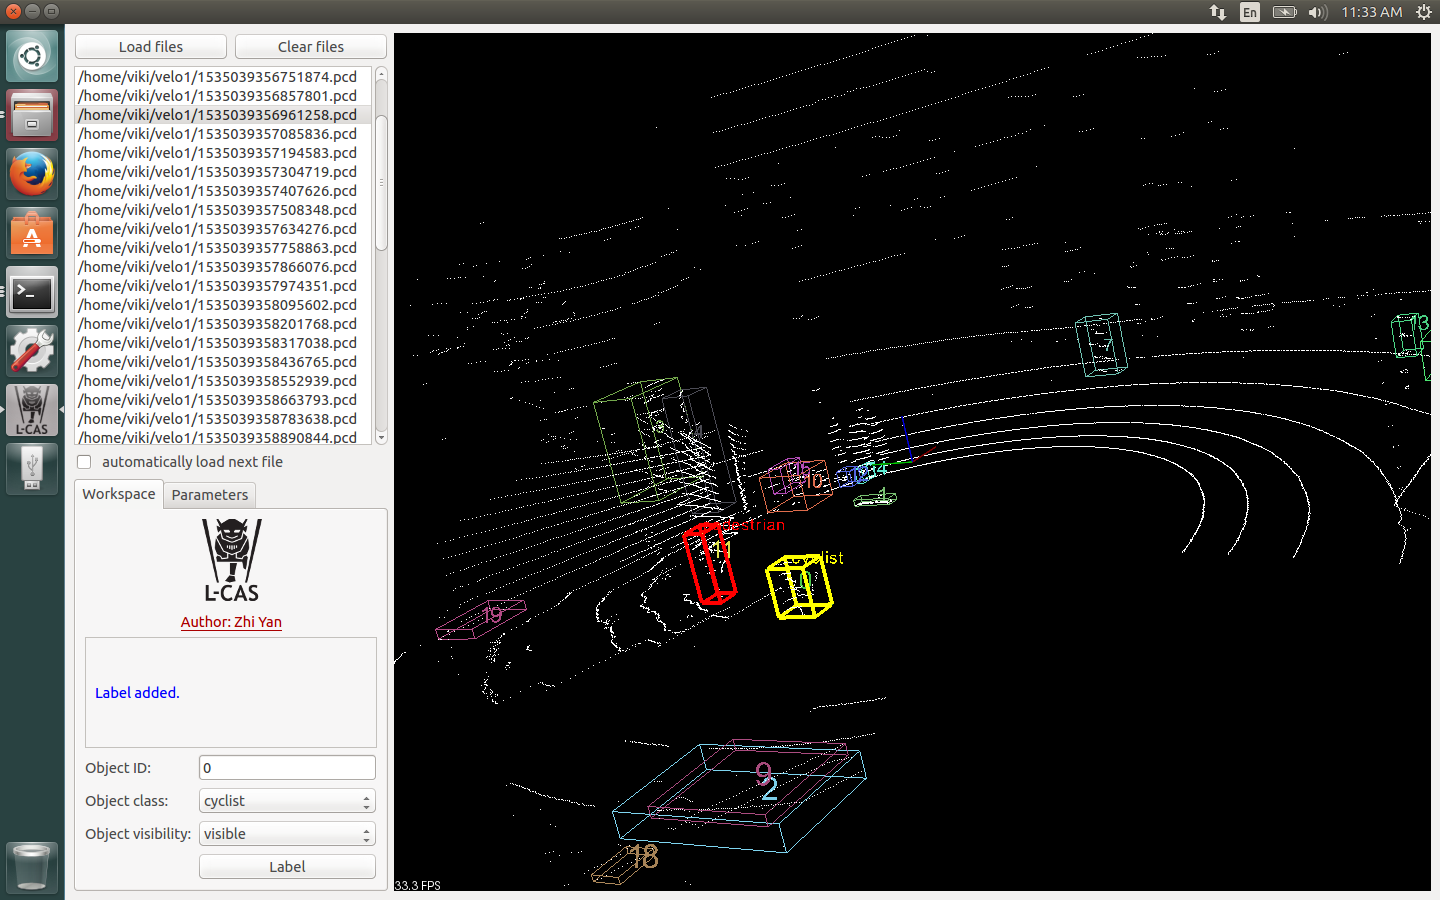
\includegraphics[width=\linewidth]{images/annot.png}
	\caption{L-CAS Annotation Tool}
	\label{fig:annot}
\end{figure}

\subsubsection{Validation}
Using the annotation tool, I annotated 500 frames to be used for validation. The output was a list of files containing object labels and their bounding boxes that would serve as the ground truth for validation. 
I then  ran VoxelNet on these frames to generate the predicted bounding boxes for different object classes.  


\section{Conclusion}
In the beginning of this section I set out to answer three important questions. Following a methodological approach I was able to establish tools to detect and characterise the context of images and point clouds. Building up on this, I was able to identify two neural networks that could potentially perform better in different contexts. 
Finally, I was able to identify a potential challenge with LiDAR only models and we were able to test whether VoxelNet would still perform given a different dataset. 
